% Copyright (c) 2014,2016 Casper Ti. Vector
% Public domain.

\chapter{比特幣交易監督系統設計}
%\pkuthssffaq % 中文测试文字。
本論文提出基於區塊鏈的支付收款監督系統(Blockchain-based Payment Collection Supervision System,BPCSS),以下簡稱BPCSS,BPCSS以密碼貨幣比特幣實作,BPCSS包含三個子系統,商店和商品信息管理子系統(Store and Merchandise Information Management Sub-System,SMIMSS)、商家移動裝置收款及交易子系統(Store Mobile payment Collection and Transaction、Sub-System,SMCTSS)、客戶端移動支付和交易子系統(Client Mobile Payment and Transaction Sub-System,CMPTSS),我們將在稍後描述這些子系統。

	\section{BPCSS數據庫設計}
		\section{原資料庫}
		基於區塊鏈的支付收款監督系統應用了四個原數據庫,分別為使用者資料庫、產品資料庫、商家資料庫、交易資料庫:

			\paragraph{店家數據庫}存儲正在審核中的企業信息或已經過審核的企業信息。存儲的信息包括商家ID,商戶名稱,商戶位置,商戶的數字貨幣地址以及GPS坐標。
			\paragraph{產品數據庫}只有授權用戶才能登錄添加或修改交易產品信息。產品數據庫內容包括產品標識號,產品名稱,產品說明,日期和價格等相關信息。
			\paragraph{交易數據庫}記錄包括交易序列號,產品識別號碼,產品交易金額,商戶數字貨幣收款人地址,消費者數字貨幣支付地址,商戶ID和最後確認字段的值。
			\paragraph{使用者資料庫}儲存所有使用者資訊,包括政府、商家及顧客之個人帳戶資訊的資料庫,而使用者密碼則以雜湊的方式保存,以增加用戶安全性。

		\section{關聯資料庫}
		\paragraph{商家-用戶資料庫}本資料庫儲存各個商家擁有的職員資訊,包括各店家的商店編號、使用者編號及身分編碼。
		\paragraph{商家-產品資料庫}此資料庫儲存各家公司當前商品存貨資訊,由商店編號、產品編號及產品庫存所組成。
		\paragraph{商家-交易資料庫}本資料庫記錄著每一筆交易的經手人是誰,並由交易編號、店家序號,及使用者序號組成。

	\section{商店和商品信息管理子系統(SMIMSS)}
	在提出的基於區塊鏈的支付收款監督系統架構中,商家需要在以下4個步驟中對商店和商品信息管理子系統(SMIMSS)進行註冊:

	\begin{figure}[h]
		\centering
		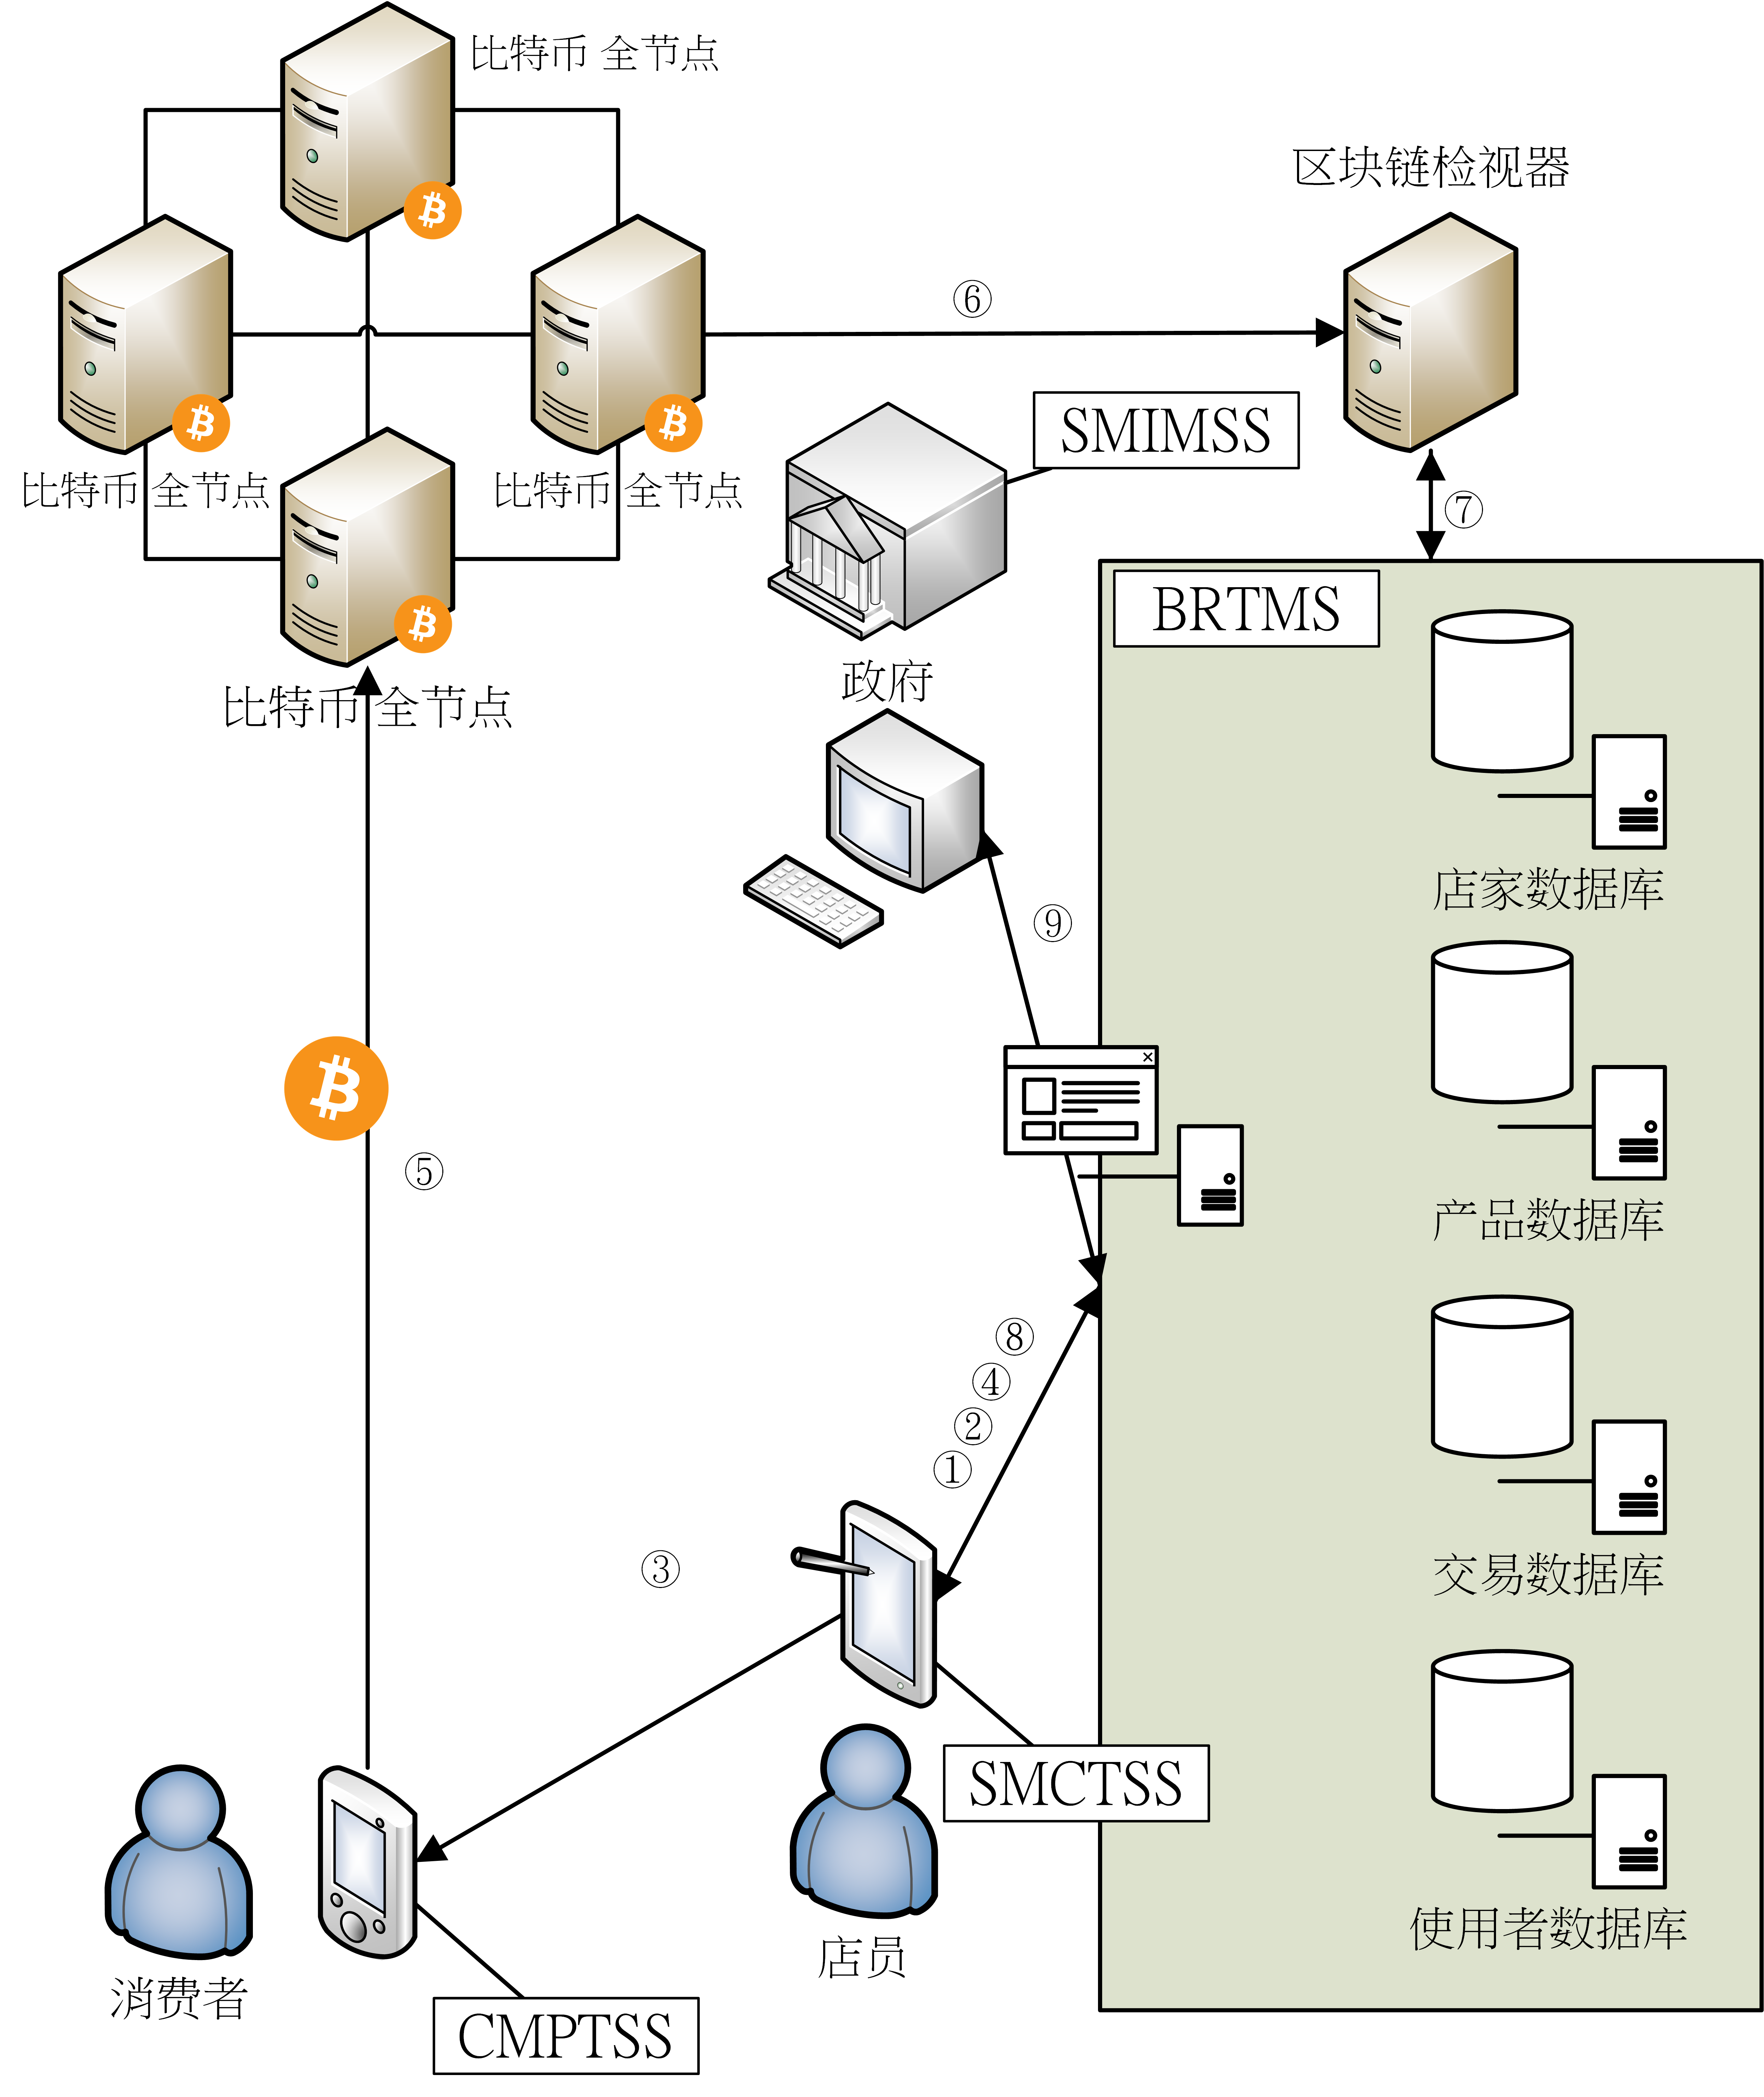
\includegraphics[width = 0.6\textwidth]{fig4.png}
		\caption{fig4}\label{fig4}
	\end{figure}

		\paragraph{第一步}商戶必須在BPCSS註冊一個帳戶,並附有政府法規的商業證明。
		\paragraph{第二步}基於區塊鏈的支付收款監督系統將自動向相應的政府金融監管機構提交商業申請,以審查該商店的數字貨幣交易業務。
		\paragraph{第三步}如果政府批准商店的數字貨幣業務申請,服務器將激活商家在該收集監控系統中創建的商店帳戶。
		\paragraph{第四步}商家可以自由地登錄賬戶並添加商家想要出售的產品,並檢查他們的數字貨幣交易數據,例如產品庫存和產品交易記錄。

	\section{BPCSS運作流程}
	密碼貨幣交易的實際在BPCSS中操作流程如圖示。 首先,我們需要連接到比特幣區塊鏈瀏覽器。建議的BPCSS監控系統可以應用區塊鏈瀏覽器來將交易活動與BPCSS中記錄的交易相匹配。 這樣的設計可以幫助BPCSS在數字貨幣交易中實現即時性和正確性。 如果直接性和正確性僅僅是來自區塊鏈探索者的結果,我們可以使用多個區塊鏈探索者進行交叉引用,以避免區塊鏈探險家公司的錯誤帶來的業務影響。 使用區塊鏈探索者的目的是快速準確地完成交易。 這是使整個交易從發行到完成的主要步驟之一。
	基於區塊鏈的支付收款監督系統中創建步驟描述如下:
		\paragraph{第一步}商家的店員將登錄到如圖3所示的先前步驟創建的帳戶,以使用手持式平板電腦或智能手機訪問SMCTSS中的服務。如前所述,在能夠登錄到系統之前,商家帳戶必須由政府機構審計。
		\paragraph{第二步}在成功登錄SMCTSS用於商戶數字貨幣流量監控系統時,移動設備將加載通過SMIMSS註冊的商店產品信息,然後創建產品目錄。商店的店員可以根據客戶的需求選擇所需的產品和數量。
		\paragraph{第三步}店員使用設備完成客戶選定商品的產品信息後。移動設備上的NFC技術可用於將產品信息從附近店員的移動設備傳遞給消費者的移動設備,而無需物理交互。然後,消費者可以很容易地將他/她自己的消費信息記錄為發票等參考。在接收從商家店員設備向顧客設備購買產品的消息的同時,顧客設備還將向商家的移動設備發送其自己的比特幣支付地址的消息。
		\paragraph{第四步}商家的手持設備收到客戶確認購買所選產品的相應信息後,會將交易信息的副本發送給SMIMSS監控系統。消費者信息包括交易序列號,商戶ID號碼,商品號碼,購買的商品的數量,以及數字貨幣的收款人地址以及消費者的支付地址。
		\paragraph{第五步}收到消費者交易信息後,此確認將支持以比特幣等數字貨幣支付。同時,此次交易的數字貨幣將發佈到比特幣網絡中進行驗證和記錄。
		\paragraph{第六步}區塊鏈瀏覽器將開始分析在比特幣網絡中緩存的所有交易以及區塊鏈中記錄的交易。
		\paragraph{第七步}擬議的交易監控系統BPCSS將向區塊鏈探索者提出請求。這個請求數據不僅包括存儲在BPCSS中的交易副本的數字貨幣收款人地址(如圖3的第4步所述),還包括客戶預期付款的數字貨幣支付地址。區塊鏈瀏覽器使用請求數據來檢查交易是否存儲在區塊鏈中,或者交易還在等待確認。如果交易已被確認並存儲在區塊鏈中,則交易數據庫中“交易確認”字段的值將更改為“1”,否則其默認值為零。
		\paragraph{第八步}當“交易確認”字段中的值為“1”時,“交易已完成”消息可發送至商店平板電腦上運行的商店和商品信息管理子系統(SMCTSS)。
		\paragraph{第九步}政府財政監督部門可以審查擬議BPCSS中的所有交易信息,以作為稅收審計參考。

	
% vim:ts=4:sw=4
